\section{Product prespective}
% Describes external interfaces: system, user, hardware, software; also operations and site adaptation, and hardware constraints.
% It defines the boundaries of the system. Further details on the shared phenomena and a domain model (class diagrams, and statecharts)

The PowerEnJoy front end is only composed of a mobile app.
%There can be a website that contains only information and reminds to the link of the app in both Apple Store and Play Store, but it is not our purpose to develop it.
The system developed will not be integrated with other existing systems that managed a car-sharing service.

Also, the system will only be user based, this means no internal interface will be developed for now.
For example, it will be possible to modify the safe areas and the power grid stations only by the database interface, so editing the tables directly.
In the future some API will be provided, in order to permit the evolution of the features of the system.

The interaction with the car is managed by "HandyCar", a system that abstract all the operations related to the interaction with the car, like lock and unlock the car, know his battery level, the number of passengers and so on.


\subsection{User Interfaces}
All the interfaces shall be intuitive and user friendly. They should not
require the reading of detailed documentation to be used.

\subsubsection*{Main page}

\begin{figure}
	\centering
	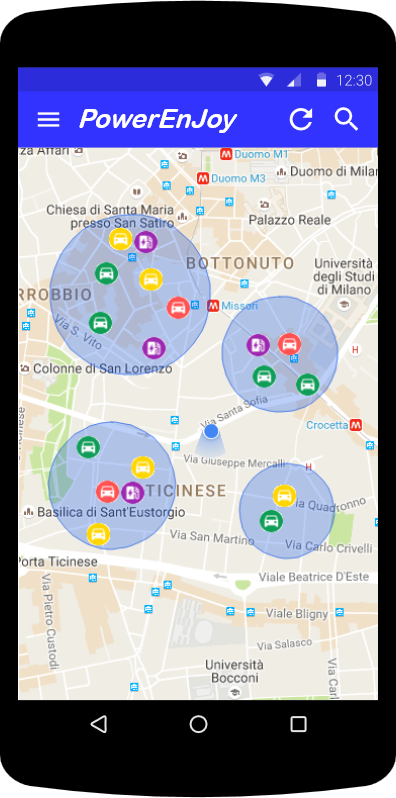
\includegraphics[width=\textwidth,height=\dimexpr\textheight-4\baselineskip-\abovecaptionskip-\belowcaptionskip\relax,keepaspectratio]{overall_description/mockup/main_page.png}
	\caption{Main page.}
	\label{fig:mockup_main_page}
\end{figure}

In figure \ref{fig:mockup_main_page} is represented the first page that is shown to the user if it logged in to the system before.

From this page a user can search for the nearest available car having a quick look to their battery level, too.

The legend of the battery level is the following:
\begin{description}
	\item[red:] battery level from 1\% to 19\%;
	\item[yellow:] battery level from 20\% to 49\%;
	\item[green:] battery level from 50\% to 100\%.
\end{description}

\subsubsection*{Car selection}

\begin{figure}
	\centering
	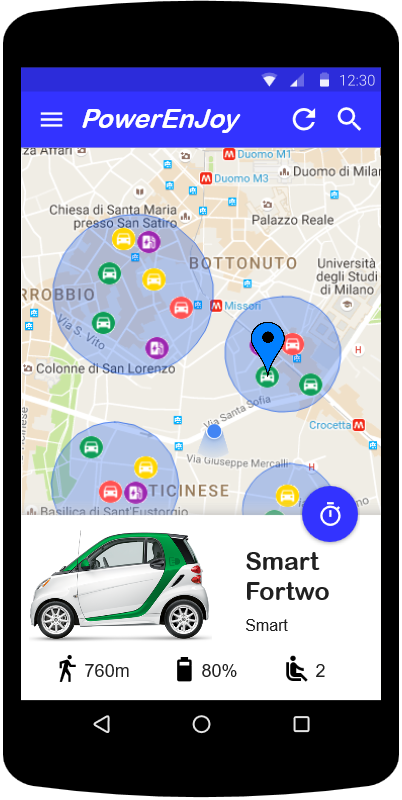
\includegraphics[width=\textwidth,height=\dimexpr\textheight-4\baselineskip-\abovecaptionskip-\belowcaptionskip\relax,keepaspectratio]{overall_description/mockup/car_selection.png}
	\caption{Car selection.}
	\label{fig:mockup_car_selection}
\end{figure}

From the Main page, when the user select a car a bottom sheets slides up from the bottom of the screen to reveal the car information and a marker will appear over the car that he/she selected. You can reserve the car by clicking on the blue bottom with the timer icon (a yes/no confirmation will appear). You can see this screen in figure \ref{fig:mockup_car_selection}.

\subsubsection*{Car unlock}

\begin{figure}
	\centering
	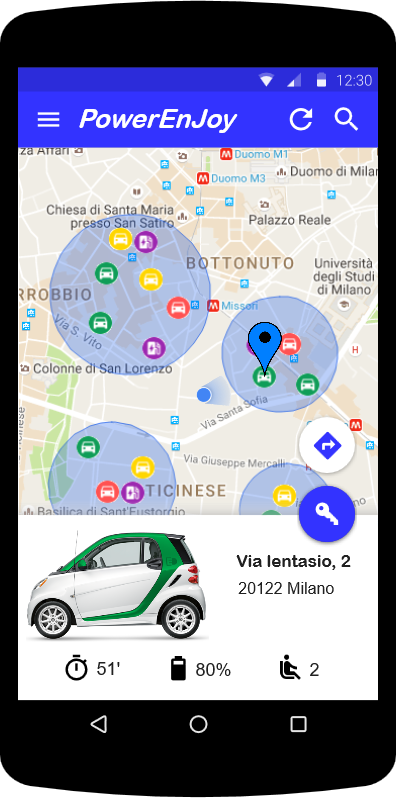
\includegraphics[width=\textwidth,height=\dimexpr\textheight-4\baselineskip-\abovecaptionskip-\belowcaptionskip\relax,keepaspectratio]{overall_description/mockup/car_unlock.png}
	\caption{Car unlock.}
	\label{fig:mockup_car_unlock}
\end{figure}

After the reservation of the car, you can see how the screen changes in figure \ref{fig:mockup_car_unlock}. The user can find indications to the car by pressing the white button that appears and when he/she is near to the car he/she can press the button with the key. Then, to unlock the car, his/her password will be required.

\subsection{Hardware interfaces}
In the system there are the following hardware interfaces:
\begin{description}
	\item [Panic button:] a button that is present in every car and can be pressed by the user to report that there something wrong with the mechanical aspects of the car;
	\item [GPS:] it's used to track the position of cars and users;
	\item [HandyCar Board:] a board to which all the actuators and sensors of the car are connected. The sensors system that detects how many passengers there are in the car it's connected to this board too, so the board can memorize the maximum number of passengers of the current ride.
\end{description}

\subsection{Software interfaces}
The mobile app will be developed both for IOS and Android, so the system will use the API of these operating systems to access to the GPS of the smartphone and maps.

Furthermore, the HandyCar Board provides some simple API, in order to control the board remotely through the Internet.

The other software interfaces that we have are the external payment	gateway and the motorization gateway.




